% Mechanical Systems and Signal Processing -- research paper.
% Compile: pdflatex main; bibtex main; pdflatex main; pdflatex main   (elsarticle + elsarticle-num)
% Every table in tables/ is generated by paper/make_tables.py; every figure by a script in paper/figures/.
\documentclass[preprint,3p,times]{elsarticle}

\usepackage{amsmath,amssymb}
\usepackage{booktabs}
\usepackage{graphicx}
\usepackage[table]{xcolor}
\usepackage{url}
\usepackage[hidelinks]{hyperref}
\usepackage{siunitx}
\sisetup{detect-all,group-separator={,}}

\journal{Mechanical Systems and Signal Processing}

\begin{document}

\begin{frontmatter}

\title{Bearing-wise evaluation of source-free domain adaptation: leakage, bearing-identity memorisation and the ceiling of
physics-gated pseudo-labels}

%% ANONYMOUS FOR NOW. Before submission: real author list, affiliations, corresponding author and e-mail here, and the
%% CRediT statement in sections/99_declarations.tex.
\author[a]{Anonymous}
\address[a]{Affiliation withheld}

\begin{abstract}
Source-free domain adaptation (SFDA) reports near-ceiling accuracy for rolling-bearing diagnosis, yet the evaluation
protocols behind those numbers place the same physical bearings on both sides of a transfer task. We re-evaluate a published
SFDA method (SDALR) for cross-condition transfer using a paired design in which only bearing overlap changes. On Paderborn,
bearing-disjoint targets lower mean accuracy from \SI{94.1}{\percent} to \SI{56.8}{\percent} on two mechanical folds and by a
median of 36.2 percentage points (range 8.2--61.6, $p=0.001$) over ten pre-registered random bearing splits; on a second rig
(HUST bearing) six type-disjoint splits lose a median of 33.5 points. SHOT collapses likewise, and so does a random forest on
ten time-domain statistics that uses no adaptation at all --- that baseline exceeds the adapted model on bearing-disjoint
targets by a median of 8.9 points. Saved predictions show the adapted model labelling each physical bearing as a whole, and a
probe recovers the individual bearing among same-class bearings in 507 of 508 held-out recordings. An oracle filter that keeps
only correct pseudo-labels recovers a median \SI{82}{\percent} of the collapse, which bounds what any pseudo-label filter can
achieve. Kinematic envelope gates, selected by their false acceptance on 480 real healthy recordings (at most
\SI{2}{\percent}, against \SI{45}{\percent} for a raw-spectrum band rule of the kind used in recent physics-guided SFDA), add
4--7 points in paired comparisons and close a median \SI{19}{\percent} of that gap, while the raw-spectrum rule lowers
accuracy. We conclude with the evaluation evidence a source-free bearing-diagnosis result should carry.

\end{abstract}

\begin{highlights}
\item Bearing-disjoint targets cut source-free adaptation accuracy by 37 points.
\item The collapse replicates on a second rig and for SHOT and a non-adaptive forest.
\item Source features identify same-class bearings in 507 of 508 held-out recordings.
\item Physics gates give paired gains of 4--7 points, bounded by a perfect-filter ceiling.
\item A non-adaptive random forest beats the adapted model by a median 8.9 points.
\end{highlights}

\begin{keyword}
rolling bearing \sep source-free domain adaptation \sep data leakage \sep bearing-wise evaluation \sep
pseudo-label gating \sep envelope analysis
\end{keyword}

\end{frontmatter}

\section{Introduction}
\label{sec:intro}

Rolling-element bearings fail in service, and the vibration signature of a spall or a crack is well understood: an impact
train at a kinematic frequency fixed by the bearing geometry and the shaft speed, modulated by load and smeared by cage slip
\cite{randall2011}. Condition-monitoring practice turns that signature into a decision --- replace the bearing, or leave it
--- and the value of an automated diagnosis is the reliability of that decision on a machine the diagnostic system has not
seen before.

Data-driven diagnosis has moved towards transfer learning to meet exactly that requirement. Unsupervised domain adaptation
transfers a model trained under one operating condition to another without target labels \cite{zhao2021udtl}, and source-free
domain adaptation (SFDA) goes further: during adaptation only the trained source model and unlabelled target recordings are
available, which suits a fleet operator who cannot ship raw data between sites \cite{liang2020shot,sdalr2025}. Reported
accuracies are high. In a survey of 18 bearing-diagnosis papers published in 2025, every one reported above
\SI{94}{\percent} and six reported \SI{100}{\percent} \cite{vieira2026}. None of the 18 evaluated on bearings that were
absent from training.

That omission matters because a vibration dataset carries two kinds of information at once. One is the fault physics that
should transfer: the impact train at the outer-race or inner-race passing frequency. The other is the acoustic identity of an
individual specimen --- its clearance, mounting, surface finish, resonances and the particular way its damage was produced.
When a model may see the same physical bearing in training and in test, identity is sufficient to score well, and no
experiment in that protocol can tell the two apart. Splitting by physical bearing removes the shortcut, and in supervised
single-bench settings it has already been shown to change conclusions \cite{hendriks2022,wheat2024leakage,vieira2026}.

SFDA deserves separate scrutiny, for a reason specific to how it works. Adaptation is driven by the source model's own
predictions on target data: pseudo-labels, centroids or neighbourhood structure, refined over iterations. If the source
representation has learned to recognise the individual bearings it was trained on, then on a new bearing there is nothing
correct to refine --- the procedure sharpens a decision that was never about the fault. Whether this happens, how much
performance it costs, and whether anything can repair it are empirical questions that a leaky protocol cannot ask.

Physics offers a natural remedy and is increasingly used as one: characteristic-frequency evidence can filter pseudo-labels
during adaptation, as in the EAGLE module of Bio-SFDA \cite{yoon2026biosfda} or the consistency validator of PCTL
\cite{pctl2026}. Such filters are usually justified by end accuracy on the same leaky protocols. Their false acceptance on
healthy bearings --- the rate at which they certify a fault that is not there, which is what makes them safe or unsafe inside
an adaptation loop --- is rarely reported, and the amount of damage a perfect filter could repair has not been measured.

This paper follows one thread through those questions, with the evaluation apparatus fixed before the experiments were run.

\begin{enumerate}
  \item \textbf{How much survives.} A paired design holds the source model and the target operating condition fixed and
        changes only bearing overlap, so the leaky--clean difference is attributable to that overlap alone
        (Section~\ref{sec:protocol}). We measure it on two mechanical folds, ten pre-registered random bearing splits and a
        second test rig, for two SFDA methods and for non-adaptive baselines (Sections~\ref{sec:res-collapse}
        and~\ref{sec:res-second}).
  \item \textbf{What the model learned instead.} Saved per-window predictions and a linear probe on the frozen source
        features locate the failure: the representation separates same-class bearings almost perfectly, and the adapted
        model assigns one label to each physical bearing (Sections~\ref{sec:res-mechanism} and \ref{sec:res-probe}).
  \item \textbf{What could be repaired at best.} An oracle filter that keeps only correct pseudo-labels splits the collapse
        into a filter-recoverable part and a part carried by the source representation, which bounds every pseudo-label
        filter, physical or statistical (Section~\ref{sec:res-decomp}).
  \item \textbf{What physics gating actually buys.} Four gates are compared by false acceptance on 480 real healthy
        recordings and over their full operating curves, then inserted into the adaptation loop and evaluated as paired
        differences against the oracle ceiling (Section~\ref{sec:res-gating}).
  \item \textbf{Kinematic housekeeping.} We report per-manufacturer Paderborn geometry, a measured cage-slip distribution
        that settles when 6203 fault lines can lock onto shaft orders (Section~\ref{sec:res-slip}), and dataset corrections
        in the supplementary material.
\end{enumerate}

We claim no new network, no new detector and no new adaptation algorithm. Statistical envelope thresholds are established
\cite{borghesani2013,randall2011}, harmonic-coordinate features close to the ones used here were published by Matania et al.
\cite{matania2025}, and class-conditional adversarial invariance is standard in domain generalisation \cite{li2018ciddg}. The
contribution is the leakage-controlled evaluation of source-free adaptation, the measured mechanism behind its failure, the
ceiling that bounds physics gating, and the evidence a result in this area should carry before it is believed.

\section{Background and related work}
\label{sec:background}

\subsection{Leakage in bearing-diagnosis evaluation}

Hendriks, Dumond and Knox showed that the conventional condition-wise split of the CWRU data places the same physical
bearings in training and test sets, and proposed benchmarking with independent sets of bearings \cite{hendriks2022}. Wheat et
al.\ compared run-to-run, day-to-day and part-to-part splits for classical pipelines and found the gap between them large
enough to change method rankings \cite{wheat2024leakage}. Vieira et al.\ generalised bearing-wise partitioning across four
datasets, reformulated diagnosis as multi-label detection and measured the inflation caused by bearing- and
segmentation-level leakage over 100 evaluation splits \cite{vieira2026}; their study is supervised, and cross-domain and
source-free settings are stated as out of scope. Matania et al.\ \cite{matania2024leakage} make the same case for
condition-based maintenance generally, showing how test--training separation should be constructed. Knap et al.\ published a
leakage-safe cross-domain benchmark on CWRU and Paderborn with six fixed source--target scenarios
\cite{knap2026leakagesafe}; separation there is enforced at
\emph{recording} level, which removes window leakage but still permits the same physical bearing on both sides of a transfer
task, and no source-free method is evaluated.

Beyond this field, Kapoor and Narayanan \cite{kapoor2023leakage} document leakage as a systemic failure across 17
scientific disciplines and give the taxonomy we adopt, and Geirhos et al.\ \cite{geirhos2020shortcut} name the underlying
learning behaviour: a shortcut that succeeds on the benchmark and fails under the intended shift.

This paper takes the bearing-wise principle from that line of work and applies it where it has not been applied: to
source-free adaptation, with the source model shared between the leaky and the clean target so that the two differ in
bearing overlap and nothing else, and with the split treated as the statistical unit.

\subsection{Source-free domain adaptation for bearings}

SHOT established the template on which most later methods build: freeze the source classifier, maximise information at the
target and refine centroid-based pseudo-labels \cite{liang2020shot}. SDALR extends it by separating reliable from unreliable
target predictions, using the reliable ones as supervision and the unreliable ones through an entropy term, and reports
\SI{96.8}{\percent} mean accuracy across Paderborn operating conditions \cite{sdalr2025}. Jeong et al.\ combine
speed-normalised order spectra with a variational autoencoder and test-time training, and find that order normalisation alone
accounts for most of their target gain \cite{jeong2025}. Published audits of SFDA stability in this field address other
failure modes, such as collapse under industrial noise, rather than bearing overlap. In all of this work the target domain is
a different operating condition of the same physical bearings.

\subsection{Physics priors inside adaptation}

Characteristic frequencies computed from geometry and speed are the natural prior for bearing diagnosis, and recent
physics-guided methods use them to steer adaptation. PCTL scores predicted classes against envelope-spectrum energy at
characteristic frequencies and trains a confidence predictor, using a small set of labelled target data \cite{pctl2026}.
Bio-SFDA gates and weights pseudo-labels with band-energy and signal-to-noise predicates at BPFO, BPFI and BSF computed on a
short-time Fourier transform, with thresholds adapted online from unlabelled target statistics \cite{yoon2026biosfda}. These
modules are evaluated through end accuracy; the rate at which they accept a fault label on a healthy bearing is not reported.
Because the Bio-SFDA task definition for Paderborn cannot be reconstructed from the article --- a ball class is listed, and
the Paderborn real-damage set contains no rolling-element damage, and the split is not described --- we evaluate the gating
\emph{mechanism as described, as we implemented it}, and make no comparison against the accuracy reported there.

\subsection{Envelope analysis and the statistics of detection}

The squared envelope spectrum is the standard carrier of second-order cyclostationary bearing signatures \cite{randall2011},
usually after a band selection such as the fast kurtogram \cite{antoni2007kurtogram} and, where discrete components
dominate, after discrete/random separation. Borghesani et al.\ derived the statistics of the squared envelope spectrum under
coloured noise and the corresponding thresholds for testing cyclostationarity \cite{borghesani2013}. The gates compared here
are built from those ingredients; none of them is claimed as new. Matania et al.\ project order-domain envelope spectra onto
kinematic harmonic positions to obtain a machine-invariant representation \cite{matania2025}, which is the same idea as the
harmonic coordinates used internally by our comb tests, and is cited as such rather than claimed.

\subsection{Invariance to a nuisance that carries the label}

Removing a nuisance factor from a representation by adversarial training is standard, but when the nuisance carries label
information, unconditional invariance conflicts with classification: aligning the marginal feature distribution under label
shift induces concept shift and, at the invariant optimum, mixes the classes \cite{liu2021labelshift}. Class-conditional
adversaries restore compatibility by removing the nuisance \emph{within} each class \cite{li2018ciddg}, and
subject-adversarial training plays the same role in EEG decoding \cite{ozdenizci2020eeg}. A bearing source set is the extreme
case of the conflict, because each physical bearing carries exactly one fault class, so class is a deterministic function of
bearing identity. Section~\ref{sec:res-probe} measures how strongly that identity is present; the corresponding remedy is
left as future work and is not claimed here.

\section{Test rigs, bearings and kinematics}
\label{sec:data}

\begin{table}[htbp]
\centering
\caption{Test rigs and recordings used in this study. Bearings are physical bearings, not fault classes.}
\label{tab:datasets}
\small
\setlength{\tabcolsep}{4pt}
\begin{tabular}{lllrrl}
\toprule
Dataset & Bearings used & $f_s$ (kHz) & Record (s) & Conditions & Role \\
\midrule
Paderborn (PU) \cite{lessmeier2016} & 6 healthy, 5 outer, 6 inner (real) & 64 & 4 & 4 (2 used) & adaptation, gating, slip \\
HUST bearing \cite{thuan2023hust} & 5 types $\times$ \{healthy, inner, outer\} & 51.2 & 10 & 3 loads & second-rig replication \\
CWRU \cite{smith2015} & 6205 drive end, 6203 fan end & 12 & $\approx$10 & 4 loads & slip, contamination \\
UORED-VAFCLS \cite{sehri2023uored} & 20 bearings, natural faults & 42 & 10 & 1 & gate safety (suppl.) \\
JNU \cite{li2013jnu} & as published & 50 & 20 & 3 speeds & reproduction only \\
\bottomrule
\end{tabular}
\end{table}


Table~\ref{tab:datasets} lists the recordings used. \textbf{Paderborn} \cite{lessmeier2016} carries the adaptation
experiments: its real-damage set holds 6 healthy, 5 outer-race and 6 inner-race bearings, each recorded 20 times at four
operating conditions, which is the only public combination of several physical bearings per class \emph{and} several
operating conditions per bearing that allows the paired design of Section~\ref{sec:protocol}. We use the three conditions
that share a nominal speed of \SI{1500}{rpm} and differ in load and radial force, denoted A1 (N15\_M01\_F10), A2
(N15\_M07\_F04) and A3 (N15\_M07\_F10); the fourth condition (N09, \SI{900}{rpm}) enters only the gate and slip analyses.
\textbf{HUST bearing} \cite{thuan2023hust} provides the second-rig replication: one physical bearing per class for each of
five bearing types (6204--6208) at three motor loads, giving the same three-domain, six-task structure with the same label
space. \textbf{CWRU} \cite{smith2015} and \textbf{UORED-VAFCLS} \cite{sehri2023uored} appear in the slip measurement and in
the supplementary gate study. JNU \cite{li2013jnu} is used only to reproduce the published SDALR result.

Throughout, a \emph{bearing} means a physical specimen, identified by its dataset code (for example Paderborn KA04), not a
fault class or a damage severity. The label space is $\{\text{normal},\text{inner race},\text{outer race}\}$: Paderborn's
real-damage set contains no rolling-element damage, so a ball class cannot be formed from it, and HUST's ball recordings are
excluded for comparability.

\subsection{Kinematics are resolved per bearing}
\label{sec:kinematics}

Characteristic orders follow from the ball count $n$, ball diameter $d$, pitch diameter $D$ and contact angle $\theta$
through $r=(d/D)\cos\theta$, giving $\mathrm{BPFO}=\tfrac{n}{2}(1-r)$, $\mathrm{BPFI}=\tfrac{n}{2}(1+r)$ and
$\mathrm{FTF}=\tfrac{1}{2}(1-r)$ in shaft orders. A bearing designation does not determine these values. Paderborn's
per-bearing documentation, distributed with the data as one datasheet per specimen rather than in the dataset paper, states
``Pitch circle diameter mm 29.05'' and ``Number of rolling elements pc. 8'' for the 26 IBU and MTK bearings, and
\SI{28.55}{\milli\metre} for the six FAG bearings, with rolling elements of \SI{6.75}{\milli\metre}. The corresponding
outer-race orders are 3.0706 and 3.0543, neither of which equals the 3.0531 of the CWRU SKF 6203 that is frequently reused
for Paderborn. We compute kinematics separately for each specimen, and no gate is computed for a bearing whose geometry its own rig does
not publish. HUST is such a case: its dataset paper gives bore, outside and ball diameters and the ball count, but not the
pitch diameter and no characteristic orders \cite{thuan2023hust}. Substituting the nominal mean diameter $(d_i+d_o)/2$
would supply the missing number, and it is worth seeing what that costs: on Paderborn, where the true value is documented,
the same substitution gives \SI{28.50}{\milli\metre} against \SI{29.05}{\milli\metre} and shifts the outer-race order by
\SI{0.58}{\percent} --- roughly twice the whole cage-slip spread measured in Section~
ef{sec:res-slip}, and enough to move
a gate window off its line. We therefore use HUST for raw windows only and report no HUST gating result. Shaft speed is taken per recording from the measured speed channel on Paderborn and from the in-file value
on CWRU; UORED's logged speed is unreliable and is discussed in Supplementary~S3.

\section{Evaluation protocol}
\label{sec:protocol}

\begin{figure}[htbp]
\centering
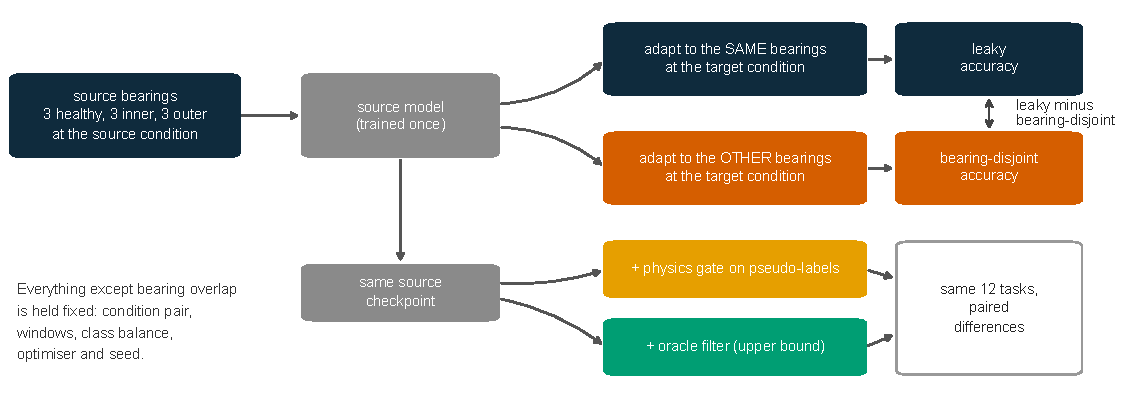
\includegraphics[width=\linewidth]{figures/fig1_design.pdf}
\caption{The paired design. One source model is trained on the source bearings at the source condition and then adapted
twice: to the \emph{same} bearings at the target condition (leaky) and to the complementary bearings at the same target
condition (clean). Both targets share the operating condition, the window contract and the class balance, so their
difference isolates bearing overlap. Gated and oracle arms reuse the same source checkpoint.}
\label{fig:design}
\end{figure}

\subsection{The paired leaky/clean design}

A source bearing set of 3 healthy, 3 outer-race and 3 inner-race specimens is trained at one operating condition. The
resulting source model is then adapted, without target labels, to two different targets at the same target condition
(Fig.~\ref{fig:design}): the \emph{leaky} target, made of the same physical bearings, and the \emph{clean} target, made of
the complementary bearings. Every other factor is held fixed --- operating condition, window length, number of windows per
class, class balance, optimiser, schedule and seed --- so the leaky--clean difference, written
$\Delta_{\mathrm{leak}}$, is attributable to bearing overlap alone. With three conditions there are six ordered condition
pairs, hence six tasks per split and per direction.

Windows are 2048 samples with 2000 windows per class, balanced across the classes and spread evenly over that class's
bearings and recordings; no window crosses a recording boundary. This window contract is inherited from the released SDALR
configuration so that the reproduction of Section~\ref{sec:res-repro} is faithful.

\subsection{Splits}

\begin{table}[htbp]
\centering
\caption{Source bearing sets on Paderborn.}
\label{tab:splits}
\small
\setlength{\tabcolsep}{4pt}
\begin{tabular}{llll}
\toprule
Split & Healthy & Outer race & Inner race \\
\midrule
fold A & K001, K002, K003 & KA04, KA15, KA16 & KI04, KI14, KI16 \\
fold B & K004, K005, K006 & KA22, KA30 & KI17, KI18, KI21 \\
\midrule
S00 & K001, K003, K004 & KA16, KA22, KA30 & KI04, KI16, KI18 \\
S01 & K002, K004, K006 & KA15, KA22, KA30 & KI04, KI17, KI21 \\
S02 & K002, K003, K005 & KA15, KA16, KA30 & KI16, KI17, KI21 \\
S03 & K002, K003, K004 & KA04, KA16, KA22 & KI16, KI18, KI21 \\
S04 & K001, K002, K006 & KA15, KA16, KA30 & KI04, KI14, KI18 \\
S05 & K003, K005, K006 & KA04, KA16, KA30 & KI04, KI17, KI21 \\
S06 & K002, K003, K006 & KA16, KA22, KA30 & KI04, KI17, KI18 \\
S07 & K003, K005, K006 & KA04, KA16, KA22 & KI04, KI14, KI16 \\
S08 & K001, K002, K006 & KA15, KA22, KA30 & KI04, KI16, KI21 \\
S09 & K002, K003, K005 & KA04, KA15, KA16 & KI16, KI17, KI21 \\
\bottomrule
\end{tabular}
\begin{minipage}{\linewidth}\vspace{2pt}\footnotesize The clean target of each row is the complement within the real-damage pool (6 healthy, 5 outer-race, 6 inner-race); the leaky target is the same bearings at the target operating condition. S00--S09 were drawn uniformly without replacement from the 4{,}000 possible 3/3/3 draws with a seed fixed before any run.\end{minipage}
\end{table}


Two families of splits are used on Paderborn (Table~\ref{tab:splits}). The two \emph{mechanical folds} follow a fixed rule
--- within each (damage origin, fault type) group, sort bearing codes lexicographically and assign the first half to fold A
--- and are run in both directions, which gives 12 paired tasks. Because two folds are two draws out of the 4000 possible
3/3/3 source sets, we additionally drew ten source sets uniformly without replacement from those 4000, excluding fold A,
with the random seed and the draw list fixed in version control before any of these runs. The \emph{split} is the
statistical unit for the ten-split analyses; tasks are the unit within a fold. On HUST the same construction uses bearing
types: the source is three of the five types and the clean target is the other two, for six pre-registered splits.

\subsection{Adaptation variants}

SDALR is run from its released code with two checkpoint policies. \texttt{as\_released} keeps the released selection rule,
which compares target accuracy against its initial value and therefore consults target labels; \texttt{final\_checkpoint}
takes the last iterate and touches no target label at any point. All headline numbers use \texttt{final\_checkpoint};
\texttt{as\_released} is reported once, in Section~\ref{sec:res-collapse}, to quantify what target-label checkpoint
selection contributes. SHOT is implemented on the same backbone, data pipeline and schedule, with a frozen classifier head,
information-maximisation loss and centroid pseudo-labels recomputed each epoch, and is evaluated at the last iterate.

\subsection{Gating, pairing and the oracle ceiling}

A gate returns one verdict per \emph{recording}, in $\{\text{silent},\text{inner race},\text{outer race}\}$, which every
window of that recording inherits; silence is not a healthy verdict. Inside the adaptation loop the verdict acts on the
method's own pseudo-label step: where the gate speaks, a pseudo-label is kept only if it agrees with the verdict, and is
otherwise withheld from the supervised term; where the gate is silent, the method is unchanged. The \emph{oracle filter}
replaces the verdict by the true label, keeping only correct pseudo-labels, and therefore measures what a perfect
pseudo-label filter could achieve within the same adaptation procedure.

All arms of a comparison --- ungated, each gate, oracle --- run in the same job from the same source checkpoint with the
same seed, so the comparison is paired. We verify this from the logs rather than asserting it: the pre-update accuracy on
the target, recorded before any adaptation step, is identical across arms in every task. Effects are therefore reported as
distributions of per-task differences, not as differences of means.

The collapse is decomposed as
\begin{equation}
\underbrace{a_{\mathrm{leaky}}-a_{\mathrm{clean}}}_{\text{total}}
=\underbrace{\left(a_{\mathrm{oracle}}-a_{\mathrm{clean}}\right)}_{\text{filter-recoverable}}
+\underbrace{\left(a_{\mathrm{leaky}}-a_{\mathrm{oracle}}\right)}_{\text{not filter-recoverable}},
\label{eq:decomp}
\end{equation}
where $a$ denotes accuracy under the arm named in the subscript. The second term is what no pseudo-label filter can reach,
because it remains when every kept pseudo-label is correct.

\subsection{Statistics and pre-registration}

Effects are paired differences. Within a fold, however, the twelve tasks share source checkpoints and bearing sets, so
treating them as independent units overstates the evidence. We therefore report every primary effect three ways: the
task-level one-sided Wilcoxon signed-rank test (descriptive only), a bootstrap that resamples whole clusters, and an exact
permutation test that flips the sign of entire clusters. The cluster is the source fold for the fold experiments and the
split elsewhere. With two folds an exact cluster-level test cannot fall below $p = 0.25$, so \emph{the fold experiments are
descriptive and the ten random splits carry the inference}. Across the family of primary tests, cluster-level $p$-values are
adjusted by the Benjamini--Hochberg procedure \cite{benjamini2001}; the collapse and the gate gain over ten splits survive
adjustment ($p_{\mathrm{BH}} = 0.005$ and $0.007$). Intervals on record-level rates use a bearing-cluster bootstrap, because
recordings of one bearing are not independent.

Arms are never crossed between jobs. Running one configuration twice gives slightly different numbers (up to 1.6~pp on a
fold mean, from non-deterministic GPU reductions), so each comparison uses the arms produced inside a single job: the
leaky--clean contrast comes from the fold job, and the gated and oracle arms are compared against the ungated arm of the
gating job. Both values are reported where they differ.

Every hypothesis, decision rule, arm and budget in this paper was written into a versioned protocol before the
corresponding runs, including the gate operating points used in Section~\ref{sec:res-gating} ($z = 10$ for the envelope
rule, $\alpha = 0.05$ for the comb tests), which were fixed before any gate was evaluated; the operating-curve sweep reported later in
that section is a sensitivity analysis reported afterwards, not a selection mechanism. Each numbered change is listed
in Supplementary~S1 with what was pre-registered, what changed and why. Two consequences are visible in the paper: results
that failed their pre-registered rule are reported as such (Section~\ref{sec:res-slip}), and one planned remedy experiment
was cut for budget before any of its outcomes were seen, so no result from it appears here. Every reported number carries a
run identifier in an append-only ledger with the retained artifact and its checksum (Supplementary~S4).

\section{Physics gates}
\label{sec:gates}

Four gates are compared. All operate on a single recording, return a verdict for the label space of
Section~\ref{sec:data}, and use kinematics resolved for that specimen (Section~\ref{sec:kinematics}) with the shaft speed
measured for that recording. Cage slip is accommodated by searching a common relative offset $\delta$ within
$\pm\SI{2}{\percent}$ of the nominal orders, which is the interval that contains the slips measured in
Section~\ref{sec:res-slip}.

\paragraph{Comb test (statistical).} The signal is pre-whitened by cepstrum editing to suppress deterministic shaft
content, band-selected by the fast kurtogram \cite{antoni2007kurtogram} and converted to a squared envelope spectrum
\cite{randall2011}. For each family (outer, inner with $\pm2$ shaft sidebands, ball with cage sidebands) the spectrum is
normalised by a running-median floor and a harmonic comb of $K=5$ harmonics is scored at the best common offset. The score
is ranked against 499 surrogate combs placed at non-kinematic orders, giving a record-specific null; a family is admissible
if its surrogate $p$-value passes $\alpha/n_{\mathrm{families}}$ and at least two of its positions carry an unmistakable
line. The surviving family with the strongest evidence becomes the verdict.

\paragraph{Shaft-alias-guarded comb (comb\_v2).} As above, with two additions: a family is rejected when at least half of
its lit positions fall within 1.5 native bins of an integer shaft order, and ties are arbitrated by the fraction of aligned
lit positions rather than by raw excess. The guard exists because on a 6203 bearing the race lines sit close to integer
shaft orders (Section~\ref{sec:res-slip}), so a strong shaft comb can light a fault family that is not there.

\paragraph{Envelope threshold rule (PCV-style).} A deliberately simple rule with no pre-whitening and no statistical null: a
harmonic counts as present if the median-normalised squared envelope spectrum exceeds a threshold $z$ anywhere inside that
harmonic's slip window, and a family is declared when at least two of its first three harmonics are present. It stands for
the family of threshold-on-envelope validators used in physics-guided adaptation.

\paragraph{Raw-spectrum band rule (EAGLE-style).} Our implementation of the mechanism described for Bio-SFDA
\cite{yoon2026biosfda}: band energy and peak-to-neighbourhood ratio at BPFO, BPFI and BSF measured on a short-time Fourier
transform of the raw signal, robustly $z$-scored across recordings, with a fault declared when the predicates pass. It
differs from the other three in operating on the raw spectrum rather than the envelope spectrum, which is the property under
test.

A gate is useful inside adaptation only if it is safe on healthy machinery: a verdict of ``inner race'' on a healthy bearing
injects a wrong pseudo-label with high confidence. We therefore characterise each gate by its false acceptance on real
healthy recordings and by its full operating curve before using any of them (Section~\ref{sec:res-gating}), rather than by
end accuracy alone.

\section{Results}
\label{sec:results}

\subsection{Reproduction}
\label{sec:res-repro}

Before changing anything we reproduced the published method from its released code on its own tasks. On JNU the mean
accuracy over the six condition pairs is \SI{98.03}{\percent} against \SI{98.50}{\percent} reported; on Paderborn it is
\SI{96.20}{\percent} against \SI{96.78}{\percent}. The two hardest tasks bracket the published values over four seeds
(A3$\to$A2: $93.9\pm4.7$ against 97.84 reported; A1$\to$A2: $90.3\pm4.9$ against 87.03), and the seed standard deviation on
those tasks, about 5 points, exceeds many differences reported between competing methods in this literature. We treat the
method as reproduced and use the released hyper-parameters unchanged from here on.

\subsection{What survives bearing-disjoint evaluation}
\label{sec:res-collapse}

\begin{table}[htbp]
\centering
\caption{Paderborn: accuracy (\%) of SDALR (final checkpoint, seed 2024) on leaky and bearing-disjoint (clean) targets, with the envelope threshold gate and the oracle pseudo-label filter. Each entry is the mean over the six condition pairs of that split.}
\label{tab:collapse}
\small
\setlength{\tabcolsep}{4pt}
\begin{tabular}{lrrrrrrr}
\toprule
Split & Leaky & Clean & $\Delta_{\mathrm{leak}}$ & Gated & Gain & Oracle & Recoverable (\%) \\
\midrule
S00 & 91.5 & 66.5 & 25.0 & 69.7 & +3.1 & 89.0 & 90 \\
S01 & 96.1 & 39.8 & 56.3 & 62.5 & +22.6 & 95.1 & 98 \\
S02 & 88.8 & 51.6 & 37.2 & 60.9 & +9.3 & 73.9 & 60 \\
S03 & 93.8 & 58.6 & 35.2 & 57.2 & -1.5 & 75.5 & 48 \\
S04 & 82.2 & 74.0 & 8.2 & 77.6 & +3.6 & 92.1 & 222 \\
S05 & 98.0 & 36.4 & 61.6 & 45.4 & +9.0 & 85.1 & 79 \\
S06 & 90.2 & 68.6 & 21.6 & 73.3 & +4.7 & 83.3 & 68 \\
S07 & 99.2 & 51.5 & 47.8 & 52.1 & +0.7 & 91.9 & 85 \\
S08 & 97.1 & 37.6 & 59.4 & 60.0 & +22.3 & 91.1 & 90 \\
S09 & 89.5 & 60.1 & 29.4 & 64.4 & +4.3 & 82.5 & 76 \\
\midrule
fold A & 88.3 & 58.4 & 30.0 & 61.2 & +4.4 & 88.5 & 101 \\
fold B & 99.9 & 55.3 & 44.6 & 62.3 & +7.0 & 76.8 & 48 \\
\bottomrule
\end{tabular}
\begin{minipage}{\linewidth}\vspace{2pt}\footnotesize Median over the ten random splits: $\Delta_{\mathrm{leak}}$ 36.2~pp (range 8.2--61.6, one-sided Wilcoxon $p=0.001$); gate gain +4.5~pp (positive in 9/10, $p=0.003$); filter-recoverable share 82\,\%. The two mechanical folds are listed below the rule and are not pooled into these statistics; for them the leaky and clean arms come from the fold job, while the gated and oracle arms come from the gating job and their gain and recoverable share are computed against that job's own ungated clean arm (56.8 and 55.3\,\% for folds A and B). Differences are computed before rounding and may differ by 0.1 from the difference of the displayed values.\end{minipage}
\end{table}


\begin{figure}[htbp]
\centering
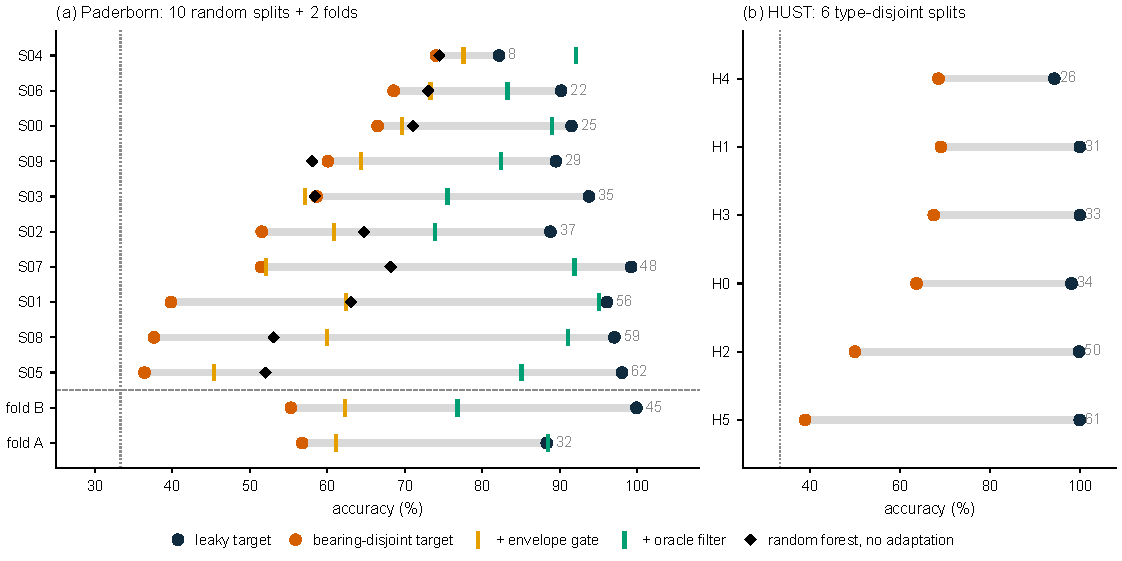
\includegraphics[width=\linewidth]{figures/fig2_collapse.pdf}
\caption{Accuracy by split on both rigs, rows sorted by the size of the collapse. Each row joins the leaky target (dark) to
the bearing-disjoint target (orange); ticks mark the same source model adapted with the envelope threshold gate (amber) and
with the oracle pseudo-label filter (green), and diamonds a random forest on ten time-domain statistics trained on the same
source windows without adaptation. The number at the right of each row is $\Delta_{\mathrm{leak}}$ in percentage points.
(a) Paderborn, ten pre-registered random bearing splits above the rule and the two mechanical folds below it; (b) HUST
bearing, six type-disjoint splits. Dotted line: three-class chance level.}
\label{fig:collapse}
\end{figure}

On the two mechanical folds, SDALR reaches \SI{94.1}{\percent} on leaky targets and \SI{56.8}{\percent} on bearing-disjoint
targets, both arms from the same job: a loss of 30.0 points with fold~A as source and 44.6 points with fold~B, 37.3 points
pooled over the 12 paired tasks. The task-level test reaches the smallest attainable value ($p=0.00024$) but treats tasks
that share source checkpoints as independent; the honest cluster-level test on two folds cannot fall below $p=0.25$, so
these two folds are descriptive and the ten random splits below carry the inference. The released checkpoint policy, which
consults target labels, gives \SI{94.7}{\percent} against \SI{57.8}{\percent}: target-label selection is worth 0.0--2.0
points and adaptation itself 2.2--5.4 points on clean targets, so neither accounts for the gap.
With fold B as source, all six leaky tasks exceed \SI{99.7}{\percent} while all six clean tasks fall between \SI{55.27}{}
and \SI{55.33}{\percent}.

Across the ten pre-registered random splits (Table~\ref{tab:collapse}, Fig.~\ref{fig:collapse}) the split-level loss has a
median of 36.2 points with a range of 8.2--61.6, which survives a cluster-level permutation test and Benjamini--Hochberg
adjustment ($p=0.001$, $p_{\mathrm{BH}}=0.005$), so the effect is not an artefact of the two mechanical folds.
The spread across splits is itself informative: which bearings happen to be in the source set moves clean accuracy between
\SI{36.4}{} and \SI{74.0}{\percent}, which is why a single split --- the norm in this literature --- cannot support a
performance claim.

\subsection{The collapse is not specific to one method}
\label{sec:res-second}

\begin{table}[htbp]
\centering
\caption{The collapse is not specific to one method: two source-free methods and four non-adaptive random forests on Paderborn, leaky versus bearing-disjoint targets (accuracy, \%).}
\label{tab:methods}
\begin{tabular}{lrrrr}
\toprule
Method & Leaky & Clean & $\Delta_{\mathrm{leak}}$ & $p$ \\
\midrule
SDALR, as released (target-label checkpoint) & 94.7 & 57.8 & 36.9 & 0.0002 \\
SDALR, final checkpoint & 94.1 & 56.8 & 37.3 & 0.0002 \\
SHOT, final iterate & 87.2 & 65.1 & 22.1 & 0.0012 \\
\midrule
Random forest, 10 time statistics & 88.8 & 63.6 & 25.2 & 0.0017 \\
Random forest, 64 spectral bands & 93.2 & 52.6 & 40.6 & 0.0002 \\
Random forest, envelope spectrum & 76.7 & 43.1 & 33.5 & 0.0002 \\
Random forest, all three feature sets & 95.4 & 60.3 & 35.1 & 0.0002 \\
\bottomrule
\end{tabular}
\begin{minipage}{\linewidth}\vspace{2pt}\footnotesize All rows use the same windows, the same two mechanical folds and the same 12 paired tasks; the random forests use no adaptation and no target data. $p$ is a one-sided Wilcoxon signed-rank test over those tasks, for which the smallest attainable value is $2^{-12}=0.00024$. Tasks within a fold share source checkpoints, so these $p$-values are descriptive; cluster-level tests are reported in Section~\ref{sec:protocol}. Differences are computed before rounding.\end{minipage}
\end{table}


\begin{table}[htbp]
\centering
\caption{Second rig: SDALR on HUST bearing, six pre-registered type-disjoint splits (accuracy, \%). The source is three bearing types; the clean target is the other two at the target load.}
\label{tab:hust}
\begin{tabular}{llrrr}
\toprule
Split & Source bearings & Leaky & Clean & $\Delta_{\mathrm{leak}}$ \\
\midrule
H0 & 6204, 6207, 6208 & 98.1 & 63.7 & 34.5 \\
H1 & 6204, 6205, 6207 & 100.0 & 69.1 & 30.9 \\
H2 & 6204, 6205, 6206 & 99.8 & 49.9 & 49.9 \\
H3 & 6205, 6206, 6207 & 100.0 & 67.5 & 32.5 \\
H4 & 6206, 6207, 6208 & 94.3 & 68.5 & 25.8 \\
H5 & 6205, 6206, 6208 & 100.0 & 38.9 & 61.1 \\
\bottomrule
\end{tabular}
\begin{minipage}{\linewidth}\vspace{2pt}\footnotesize Median $\Delta_{\mathrm{leak}}$ 33.5~pp (range 25.8--61.1, one-sided Wilcoxon $p=0.016$), which meets the replication rule fixed before the run. On this rig the clean target changes bearing size as well as bearing identity, so the shift is stronger than Paderborn's.\end{minipage}
\end{table}


Table~\ref{tab:methods} repeats the paired design for a second source-free method and for non-adaptive baselines. SHOT falls
from \SI{87.2}{} to \SI{65.1}{\percent} ($-22.1$ points, $p=0.001$). Random forests \cite{pedregosa2011sklearn} trained on the same source windows
with no adaptation at all collapse in the same way, by 25.2 points on ten time-domain statistics and by 40.7 and 33.5 points on
spectral-band and envelope-spectrum features. Bearing-disjoint evaluation therefore does not expose a weakness of one
adaptation algorithm; it exposes a property of models trained on a handful of physical bearings.

The result also replicates on a second rig. On HUST bearing (Table~\ref{tab:hust}, Fig.~\ref{fig:collapse}(b)) mean leaky accuracy
is \SI{98.7}{\percent} --- the near-ceiling figure this literature usually reports --- and mean clean accuracy is
\SI{59.6}{\percent}, with a median split-level loss of 33.5 points ($p=0.016$), meeting the replication rule fixed before
the run. On this rig the disjoint target changes bearing size as well as bearing identity, so the shift is stronger than
Paderborn's and the result is stated as identity \emph{and} geometry.

\subsection{What the adapted model does instead}
\label{sec:res-mechanism}

\begin{figure}[htbp]
\centering
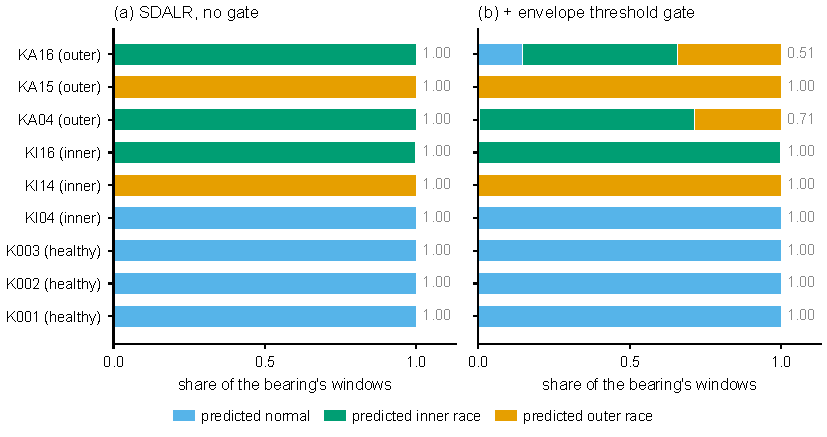
\includegraphics[width=\linewidth]{figures/fig3_purity.pdf}
\caption{Per-bearing label purity on bearing-disjoint targets: the share of a physical bearing's windows receiving that
bearing's most frequent predicted label, with the predicted label annotated. Purity 1.0 means the model gave one label to
the entire specimen.}
\label{fig:purity}
\end{figure}

Saved per-window predictions explain the numbers above. Purity is measured over all six tasks of a direction: the share of a
bearing's windows that receive its most frequent predicted label. On the bearing-disjoint targets of the fold~B direction it
is 1.000 for every bearing (Fig.~\ref{fig:purity}a). Healthy bearings are labelled healthy; among faulty bearings, KA04 and
KA16 are labelled inner race, KI04 normal and KI14 outer race. The resulting accuracy of \SI{55.3}{\percent} is arithmetic
rather than noise: with three bearings per class each labelled as a block, the three healthy bearings are right and one of
three bearings in each fault class is right, giving $5/9 = \SI{55.6}{\percent}$ up to the small imbalance in windows per
bearing. The adapted model is not making noisy per-window decisions on unseen specimens --- it is assigning one
identity-level label to each specimen.

\subsection{How much any pseudo-label filter could repair}
\label{sec:res-decomp}

\begin{figure}[htbp]
\centering
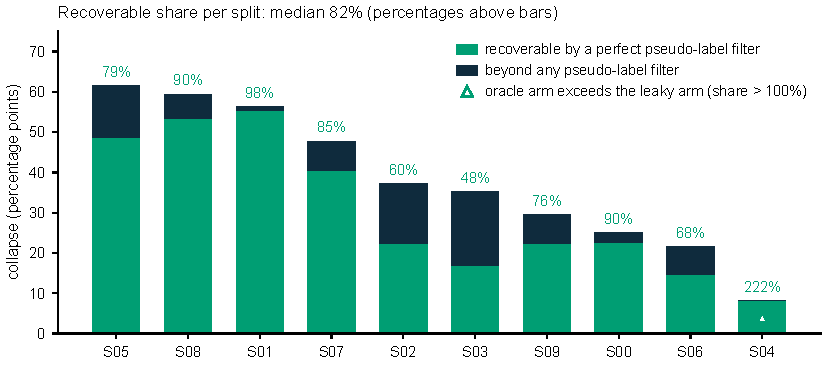
\includegraphics[width=\linewidth]{figures/fig4_decomposition.pdf}
\caption{Decomposition~\eqref{eq:decomp} per split: the part of the collapse an oracle pseudo-label filter recovers, and the
part that remains when every kept pseudo-label is correct.}
\label{fig:decomp}
\end{figure}

We apply~\eqref{eq:decomp} to the ten random splits, where all four arms of a split are produced in one job and are
therefore directly comparable. The filter-recoverable share has a median of \SI{82}{\percent} (interquartile range
68--\SI{90}{\percent}, Fig.~\ref{fig:decomp}) and varies strongly: at \SI{48}{\percent} on S03 half the collapse lies in the
source representation, while on S04 --- the mildest collapse, 8.2 points --- the oracle arm exceeds even the leaky arm, so
its share of \SI{222}{\percent} carries no upper-bound reading. The two mechanical folds behave the same way (fold~A
\SI{106}{\percent}, fold~B \SI{48}{\percent}).

The quantity being bounded should be stated precisely. The oracle arm withholds every incorrect pseudo-label and keeps every
correct one, so it bounds \emph{keep-or-withhold filters acting on this method's pseudo-label step} --- the family to which
all four gates belong. It does not bound methods that relabel samples, reweight them continuously, or change the
representation; and where it exceeds the leaky arm it is not a bound at all, but evidence that a cleaner pseudo-label set can
beat same-bearing training. With that reading, a perfect pseudo-label filter still leaves a median of about one-fifth of the
collapse untouched on this rig, and half of it on some splits.

\subsection{Physics gating: safety, paired gains and the ceiling}
\label{sec:res-gating}

\begin{table}[htbp]
\centering
\caption{Gate safety on real healthy bearings. A false acceptance is a healthy recording given a fault verdict.}
\label{tab:gates}
\small
\setlength{\tabcolsep}{4pt}
\begin{tabular}{lrrrr}
\toprule
Gate (swept parameter) & Operating point & Healthy false acceptance & Correct verdicts & At zero FA \\
\midrule
Envelope threshold rule (PCV-style), $z$ & 10 & 1/480 & 366 & 351 \\
Shaft-alias-guarded comb (comb\_v2), $\alpha$ & 0.05 & 0/480 & 312 & 312 \\
Surrogate-null comb test, $\alpha$ & 0.05 & 9/480 & 309 & -- \\
Raw-spectrum band rule (EAGLE-style), $z$ & 2 & 214/480 & 429 & 0 \\
\bottomrule
\end{tabular}
\begin{minipage}{\linewidth}\vspace{2pt}\footnotesize Population: 2{,}319 Paderborn recordings (480 healthy, 1{,}839 single inner- or outer-race). Operating points are the values fixed before the gates were evaluated. The last column sweeps each gate's parameter and reports the largest number of correct fault verdicts reachable while accepting no healthy recording. Full operating curves: Supplementary~S2. The population spans 29 physical bearings -- 6 healthy, 11 real-damage and 12 artificial-damage -- at all four operating conditions; coverage by damage origin is given in Section~\ref{sec:res-gating}.\end{minipage}
\end{table}


\begin{figure}[htbp]
\centering
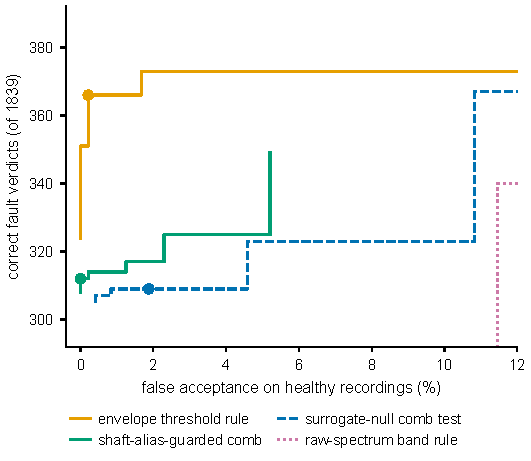
\includegraphics[width=0.8\linewidth]{figures/fig5_roc.pdf}
\caption{Gate operating curves on 2319 Paderborn recordings: correct fault verdicts against false acceptance on the 480
healthy recordings, as each gate's parameter is swept. Filled circles mark the operating points fixed before evaluation. The
envelope threshold rule lies on or above the others everywhere. The vertical range starts at 292 verdicts: the raw-spectrum
band rule returns no correct verdict below \SI{10.8}{\percent} false acceptance, and its own operating point lies at
\SI{45}{\percent}, off the right of the axis.}
\label{fig:roc}
\end{figure}

\textbf{The population.} Gate behaviour is characterised on all 2319 single-fault and healthy Paderborn recordings, spanning
29 physical bearings at all four operating conditions: 6 healthy, 11 real-damage and 12 artificial-damage (electro-discharge
machining, drilling, manual indentation). The adaptation experiments use only the healthy and real-damage bearings at three
of those conditions, so coverage is read separately by damage origin: at the pre-registered operating point the envelope
threshold rule engages 7 of the 11 real-damage bearings (209 of their 880 recordings) and 6 of the 12 artificial ones, the
alias-guarded comb 5 of 11, and the raw-spectrum rule 9 of 11 while accepting \SI{45}{\percent} of healthy recordings. Only
the real-damage figures bear on the gating results inside adaptation.

At the operating points fixed before evaluation (Table~\ref{tab:gates}), the envelope threshold rule accepts a fault label
on 1 of 480 healthy recordings, the shaft-alias-guarded comb on none, the surrogate-null comb on 9, and the raw-spectrum
band rule on 214 --- \SI{45}{\percent} of healthy machinery declared faulty. Sweeping each gate's parameter
(Fig.~\ref{fig:roc}) confirms this is not a threshold artefact: the envelope rule dominates at every false-acceptance level,
the alias guard improves the comb test, and the raw-spectrum rule is dominated everywhere. Coverage is the binding
constraint for all of them: no gate exceeds \SI{24}{\percent} correct fault verdicts before false acceptance passes
\SI{10}{\percent}, and the envelope gates engage 7 of the 11 real-damage bearings, on about a quarter of their recordings.
The operating points were fixed in the protocol before any gate was evaluated; the sweep is reported as a sensitivity
analysis, not as a selection step. Gate verdicts themselves use no target labels, but we note that an operating point
transferred to a new rig would need its own healthy recordings to be characterised, which is a deployment requirement rather
than a source-free violation.

\begin{table}[htbp]
\centering
\caption{Paired per-task effect of gating inside SDALR on the 12 bearing-disjoint tasks of the two mechanical folds (gated $-$ ungated, percentage points).}
\label{tab:gains}
\small
\setlength{\tabcolsep}{4pt}
\begin{tabular}{llrrrrrr}
\toprule
Gate & Seed & Mean & Median & Min & Max & Tasks $>0$ & $p$ \\
\midrule
Shaft-alias-guarded comb & 0 & +3.79 & +3.33 & -0.08 & +11.01 & 7/12 & 0.0078 \\
 & 1 & +4.56 & +3.28 & -0.08 & +15.45 & 8/12 & 0.0068 \\
 & 2024 & +3.73 & +3.67 & -0.05 & +8.07 & 8/12 & 0.0068 \\
\midrule
Envelope threshold rule & 0 & +7.44 & +7.57 & -0.01 & +18.02 & 9/12 & 0.0020 \\
 & 1 & +7.99 & +6.65 & -0.70 & +19.44 & 10/12 & 0.0017 \\
 & 2024 & +5.70 & +5.59 & -0.05 & +14.52 & 10/12 & 0.0010 \\
\bottomrule
\end{tabular}
\begin{minipage}{\linewidth}\vspace{2pt}\footnotesize Every arm of a comparison runs in one job on the same source checkpoint, verified from identical pre-update target accuracy in each adaptation log, so these are paired differences. The between-seed spread of the per-task gain is 1.7~pp (comb) and 2.4~pp (envelope), against 2.8~pp for ungated per-task accuracy.\end{minipage}
\end{table}


\begin{figure}[htbp]
\centering
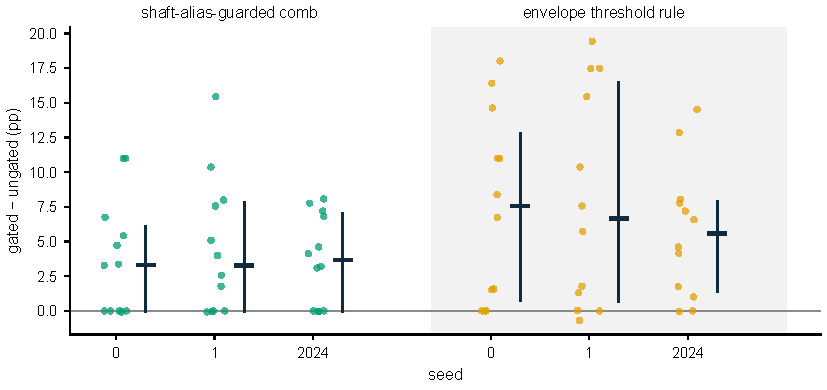
\includegraphics[width=\linewidth]{figures/fig6_gains.pdf}
\caption{Paired per-task effect of inserting each gate into the adaptation loop, over three seeds. Each point is one task;
positive values are gains over the ungated arm trained from the same source checkpoint.}
\label{fig:gains}
\end{figure}

Inside the adaptation loop the two safe gates help, consistently and modestly (Table~\ref{tab:gains},
Fig.~\ref{fig:gains}). Over three seeds the mean paired gain is $+4.03$ points for the alias-guarded comb ($p=0.007$) and
$+7.05$ points for the envelope threshold rule ($p=0.0007$), positive in every seed, and no gated task loses more than 0.70
points. The paired design matters here: the between-seed spread of the per-task gain is 1.7 and 2.4 points, against 2.8
points for ungated per-task accuracy, so an unpaired comparison of means at this scale would be uninformative. Over the ten
random splits the median gain is $+4.5$ points, positive in 9 of 10 ($p=0.003$). The unsafe raw-spectrum rule lowers
accuracy by 3.9 points, as its false-acceptance rate predicts.

Measured against the ceiling of Section~\ref{sec:res-decomp}, the envelope gate closes a median of \SI{19}{\percent} of the
oracle gap. Where it engages a bearing it does break the identity lock --- on the bearing KA04 the label purity falls from
1.00 to 0.56 and one task rises from \SI{55.3}{} to \SI{69.9}{\percent} --- but it cannot act on the bearings it never
engages, nor on the part of the collapse that no filter can reach. The modest size of the gain is therefore a property of
the problem, not of the tuning.

\subsection{Bearing identity in the source representation}
\label{sec:res-probe}

The decomposition says part of the damage is in the representation; a probe shows what is in it. On the frozen source
features we fit a logistic-regression probe with record-disjoint halves, one probe per class, each required to tell apart
the bearings \emph{within} that class --- a task that carries no class information at all. Pooled over the six source models
(two folds $\times$ three source conditions), the probe identifies the correct physical bearing in 507 of 508 held-out
recordings, against a pooled chance level of 0.35. Those 508 recordings are the ones falling in the held-out half of the
deterministic hash split, which divides the 1080 source recordings 508/572 rather than exactly in half. Individual specimens
are therefore almost perfectly encoded before adaptation begins.

Identity is not something the network invents. The identical probe on ten elementary time-domain statistics of the same
windows identifies the bearing in 508 of 508 recordings ($p < 10^{-200}$ against the same chance level): the shortcut is
already present in the raw signals. That is why non-adaptive random forests collapse in the same way, and why an adaptation
objective has no reason to prefer fault physics over specimen identity --- on a rig with three bearings per class, identity
separates the source classes as effectively as the fault signature does, at no cost to the source loss. One caveat applies
to both probes: the source model was trained on other windows of the same recordings, so they measure what the
representation encodes about bearings the model has seen, not generalisation to new specimens.

\subsection{Cage slip and the shaft-order lock of 6203 bearings}
\label{sec:res-slip}

\begin{figure}[htbp]
\centering
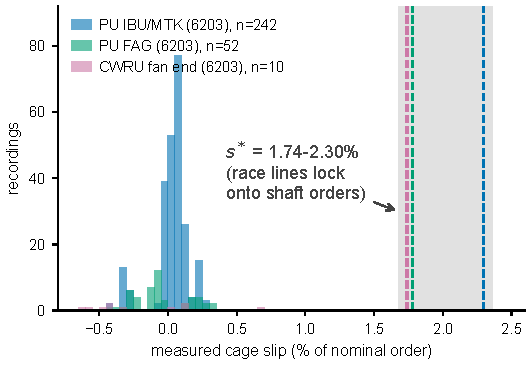
\includegraphics[width=0.85\linewidth]{figures/fig7_slip.pdf}
\caption{Measured cage slip from fault lines with per-recording measured speed. The dashed lines mark $s^\ast$, the slip at
which the outer- and inner-race lines of each 6203 geometry reach integer shaft orders simultaneously.}
\label{fig:slip}
\end{figure}

A kinematic remark closes the results, because it bears on every gate that places windows by geometry. Under the cage-slip
model $\mathrm{BPFO}(s)=(1-s)\,\mathrm{BPFO}_0$ and $\mathrm{BPFO}(s)+\mathrm{BPFI}(s)=n$, so if
$\mathrm{BPFO}_0=m+\delta$ with $m$ integer, both race lines reach integer shaft orders at the same slip
$s^\ast=\delta/\mathrm{BPFO}_0$: \SI{2.30}{\percent} for the Paderborn IBU/MTK geometry, \SI{1.78}{\percent} for the FAG
geometry and \SI{1.74}{\percent} for the CWRU fan-end bearing. Smith and Randall observed such lock-like behaviour on the CWRU fan-end bearing and
noted that it makes a definite diagnosis difficult \cite{smith2015}; the contrary view, that such lines can always be
separated given sufficient spectral resolution, appears for instance in the patent literature \cite{patent10168248}.

We tested whether it occurs in practice by measuring slip directly. Fault-line positions were fitted against the measured
shaft speed on every recording with at least two lit harmonics; on synthetic signals with injected slips of \SI{0.1}{} to
\SI{4}{\percent} the estimator recovers the truth to within \SI{0.17}{\percent}. Measured slip on Paderborn has a median of
\SI{0.06}{\percent} with a 5--95\% range of $-0.31$ to $+\SI{0.22}{\percent}$ (Fig.~\ref{fig:slip}), an order of magnitude
below $s^\ast$. Of 304 measurable 6203 recordings, three fall within tolerance of $s^\ast$, and all three fail once
shaft-order bins are masked, which identifies them as shaft pickup rather than fault lines. By the criterion fixed before
the measurement, the lock is therefore a curiosity on these rigs rather than a practical failure mode, and we report it as
such; the textbook slip range of 1--\SI{2}{\percent} does not describe these operating points. The residual offset of about
$-\SI{0.3}{\percent}$ on CWRU, where speed is logged rather than measured, bounds how precisely any fixed-kinematics window
can be placed.

\section{Discussion}
\label{sec:discussion}

\paragraph{Why the collapse is generic.} Two source-free methods, four non-adaptive random forests and two test rigs lose
between 22 and 41 points when the target bearings are disjoint from the source bearings. The probe of
Section~\ref{sec:res-probe} explains why a specific algorithm is not the culprit: the source features identify individual
specimens within a class almost perfectly, so any classifier trained on them can separate the source classes by identity.
With three bearings per class, identity is not a weak shortcut competing with fault physics --- it is a perfect one. Nothing
in an unsupervised adaptation objective penalises it, because adaptation refines the source model's own decisions rather
than questioning what they are based on. This also predicts the shape of the failure we observe: not degraded per-window
accuracy, but a confident label applied to a whole unseen specimen.

\paragraph{Why physics gating helps, and why only this much.} The gates that are safe on healthy machinery deliver 4--7
points, in every seed, in 9 of 10 splits, and essentially never cost anything. That combination --- small, consistent,
almost risk-free --- is what a correct but partial prior looks like. The ceiling analysis quantifies the ``partial''. First,
a pseudo-label filter can only repair the filter-recoverable part of the collapse, a median \SI{82}{\percent} on Paderborn
but as little as \SI{48}{\percent} on some splits. Second, a kinematic gate acts only where fault lines are actually
detectable, which on this dataset is about a quarter of the faulty bearings. The product of those two factors is a small
number, and no amount of tuning changes it. Reporting a gain without the oracle gap beside it hides exactly this.

\paragraph{Safety is a property to measure, not to assume.} The raw-spectrum band rule accepts \SI{45}{\percent} of healthy
recordings as faulty, and inside the adaptation loop it makes accuracy worse. The envelope rules accept at most
\SI{2}{\percent} and help. The ordering of the two effects is the same as the ordering of the false-acceptance rates, and
both are measurable before any adaptation experiment is run, on healthy recordings from the target rig. A physics module
introduced into an adaptation loop should be characterised this way first; end accuracy on a leaky protocol cannot
distinguish a safe prior from an unsafe one.

\paragraph{A shallow baseline belongs in every such comparison.} On bearing-disjoint targets a random forest on ten
time-domain statistics --- no adaptation, no target data, no deep network --- exceeds the adapted source-free method by a
median of 8.9 points across the ten splits, and matches the gated method. We do not present this as a better diagnostic
method; it collapses for the same reason and labels bearings as blocks in the same way. It is a calibration point. Any
claim that an adaptation procedure has learned transferable fault structure should clear the bar set by features that
encode no transfer mechanism at all.

\paragraph{Is this leakage, or simply a different task?}
A reader may object that adapting to the same physical bearings at a new operating condition is a legitimate task: the
machine is the same, only its duty point has changed, and that is a real deployment scenario for a permanently instrumented
asset. We agree, and the objection sharpens rather than weakens the argument. Two scenarios are conflated in the current
literature. In the first, the monitored bearing is present in training, and same-bearing evaluation estimates performance
honestly. In the second --- diagnosing a replacement bearing, a sister machine, or a fleet --- the specimen at test time was
never seen, and same-bearing evaluation over-estimates performance by 22--41 points on the rigs measured here. The failure is
therefore not that the published protocol is wrong in itself, but that the reported number is read as evidence for the
second scenario while being measured under the first. We use ``leakage'' in the sense of Kapoor and Narayanan
\cite{kapoor2023leakage}: information shared between training and evaluation that inflates the estimate relative to the
deployment the claim addresses. What the adapted model exploits is a shortcut in exactly the sense of Geirhos et al.
\cite{geirhos2020shortcut} --- a rule that succeeds on the benchmark and fails under the intended shift.

\paragraph{Threats to validity.} Three deserve naming. The clean and leaky targets differ in their bearing sets, so a split
where the clean bearings happen to be harder inflates $\Delta_{\mathrm{leak}}$; running both directions on the folds and ten
random splits addresses this, and the split-level spread is reported rather than hidden. The two Paderborn folds are not
perfectly symmetric (fold B's source has two outer-race bearings rather than three), which is visible in the decomposition
and is why the folds are reported separately from the ten random splits. Finally, the HUST replication changes bearing size
along with identity; it strengthens the leakage conclusion but cannot isolate identity alone, and we do not use it for any
claim about gating.

\section{What a source-free bearing-diagnosis result should carry}
\label{sec:recommendations}

The measurements above suggest six pieces of evidence that separate a transferable result from a leaky one. None requires
new hardware or a larger dataset; together they cost a few additional runs.

\begin{enumerate}
  \item \textbf{Bearing-disjoint targets.} Report accuracy on physical bearings absent from source training. If the dataset
        cannot support this --- CWRU's healthy class is effectively one specimen, for example --- say so, and treat the
        published number as an upper bound rather than an estimate.
  \item \textbf{A distribution over splits, not one split.} Which bearings fall in the source set moved clean accuracy
        between \SI{36}{} and \SI{74}{\percent} here. A single split cannot distinguish a method effect from a draw effect;
        ten pre-registered draws are affordable and make the uncertainty visible.
  \item \textbf{Paired differences for any add-on module.} Gates, regularisers and losses should be compared against the
        base method trained from the \emph{same} source checkpoint with the same seed, and reported as the distribution of
        per-task differences. The relevant variance is that of the difference, which here is roughly half the variance of
        the accuracies themselves.
  \item \textbf{An oracle pseudo-label ceiling.} One extra run per configuration, replacing the pseudo-label rule by the
        true label, converts a bare gain into a share of what was achievable and exposes the part of the gap that lives in
        the source representation.
  \item \textbf{A non-adaptive shallow baseline under the identical split.} Cheap, and it calibrates the claim: on our
        splits it beat the adapted method.
  \item \textbf{False acceptance for any physics module, measured on healthy recordings from the target rig.} A gate that
        certifies faults on healthy machinery will inject confident wrong labels; this is measurable before adaptation and
        predicted the sign of the effect in every case we tested.
\end{enumerate}

For deployment the same list reads as a risk assessment. A diagnosis system that has only been validated with the monitored
bearing present in training has not been validated for the bearing it will meet in service; the drop measured here, on two
rigs and with three model families, was 22--41 points. Where a kinematic gate is available and its false acceptance has been
characterised on healthy machinery, it is a low-risk addition --- consistent, small and essentially never harmful in our
runs --- but it is not a substitute for source data that spans enough physical specimens. For supervised models, Vieira et al.\ \cite{vieira2026} report that the number
of unique training bearings is the decisive factor for robustness. Our splits hold that number fixed at three bearings per
class, so we cannot test it here; whether a larger source pool would close the gap measured in this paper is the obvious
next experiment, and our results are consistent with their finding without being evidence for it.

\section{Limitations}
\label{sec:limitations}

The experiments concern cross-condition transfer with bearing-disjoint targets on two test rigs; no cross-machine claim is
made, and the two rigs play different roles --- Paderborn carries the full analysis, HUST only the replication of the
collapse. The HUST splits change bearing size together with bearing identity, so they confirm the effect without isolating
its cause, and HUST's unpublished pitch diameter keeps it out of every kinematic analysis.

Bearing-disjoint splits on Paderborn move more than bearing identity. Among the real-damage outer-race bearings, KA04, KA16
and KA22 carry fatigue pitting while KA15 and KA30 carry plastic deformation from indentation, so a split can place one
damage mechanism mostly on one side. The design controls the operating condition exactly, not the mechanism or the
difficulty of the individual specimen; ten random splits average over that variation but do not remove it, and a
same-condition control that varies only the bearing set would isolate it further.

Seeds and splits are traded against each other: three seeds on the two mechanical folds, one seed on each of the ten random
splits and six HUST splits. The paired design makes this affordable, since the quantity of interest is a within-job
difference, but a full seeds-within-splits grid was outside the compute budget and would tighten the split-level intervals.

Statistically, the two mechanical folds provide only two clusters, so their task-level $p$-values are descriptive and the
inference rests on the ten random splits (Section~
ef{sec:protocol}). The identity probes are measured on held-out
recordings of bearings the source model was trained on, so they establish what the representation encodes, not how it
behaves on unseen specimens.

Two source-free methods are evaluated. Neighbourhood-based methods such as NRC and AaD, and 2026-generation bearing-specific
methods, remain to be tested under this protocol; nothing here predicts that they behave differently, but nothing here
demonstrates it either.

The gating results inherit the coverage limit of envelope analysis on this dataset: the envelope gate engages 7 of the 11
real-damage bearings and fires on about a quarter of their recordings, ball faults are absent from the Paderborn real-damage label space, and no gate we tested detects rolling-element
faults on CWRU or UORED. Slip was measurable on \SI{16}{\percent} of 6203 fault recordings, namely those with at least two
lit harmonics, and UORED is excluded from the slip analysis for lack of an independent speed reference.

Finally, the raw-spectrum band rule is our implementation of a published description, not the authors' code, which was not
available; we therefore report it as a mechanism and never compare it against the accuracy published for the method it comes
from. A remedy that removes bearing identity from the source representation --- for example a class-conditional adversary,
which the probe of Section~\ref{sec:res-probe} motivates directly --- was pre-registered but cut for budget before any
outcome was observed, and is left as the obvious next experiment.

\section{Conclusions}
\label{sec:conclusions}

Source-free adaptation results for rolling bearings do not survive evaluation on bearings the source model has never seen.
On Paderborn the published method loses 37.3 points on two mechanical folds and a median of 36.2 points over ten
pre-registered random bearing splits; on a second rig it loses a median of 33.5 points; a second source-free method loses
22.1 points, and non-adaptive random forests on the same windows lose 25--41 points. Near-ceiling accuracy under the
conventional protocol and roughly \SI{60}{\percent} accuracy under a bearing-disjoint one are the same models measured two
ways.

The mechanism is identifiable rather than diffuse. The frozen source representation identifies the individual physical
bearing among same-class specimens in 507 of 508 held-out recordings, and the adapted model assigns a single label to each
unseen specimen as a whole. Adaptation cannot correct this, because it refines the source model's own decisions.

Physics helps within a ceiling that can be measured. An oracle pseudo-label filter recovers a median \SI{82}{\percent} of
the collapse, so the remainder lies in the representation and is beyond any filter. Kinematic envelope gates selected for
low false acceptance on real healthy recordings --- 1 in 480, against 214 in 480 for a raw-spectrum band rule of the kind
used in recent physics-guided adaptation --- add 4--7 points in paired comparisons, in every seed and in 9 of 10 splits,
closing about a fifth of the achievable gap, while the unsafe rule makes adaptation worse. Measured cage slip on these rigs
is about \SI{0.06}{\percent}, an order of magnitude below the slip at which 6203 race lines would lock onto shaft orders, so
that particular hazard is not active here.

For practice the implication is procedural. Bearing-disjoint targets, a distribution over bearing splits, paired
differences on a shared source model, an oracle ceiling, a shallow non-adaptive baseline and a measured false-acceptance
rate for any physics module together cost a handful of extra runs, and they are what separates a transferable diagnosis
from a memorised one.

\section*{CRediT authorship contribution statement}
% ANONYMOUS FOR NOW: replace each placeholder with a named author before submission (Elsevier CRediT taxonomy).
\textbf{Author 1:} Conceptualization, Methodology, Software, Validation, Formal analysis, Investigation, Data curation,
Writing -- original draft, Writing -- review \& editing, Visualization, Project administration.
\textbf{Author 2:} Supervision, Methodology, Writing -- review \& editing.

\section*{Declaration of competing interest}

The authors declare that they have no known competing financial interests or personal relationships that could have
appeared to influence the work reported in this paper.

\section*{Funding}
% Complete before submission, or state that no specific grant was received.
This research did not receive any specific grant from funding agencies in the public, commercial, or not-for-profit
sectors.

\section*{Data availability}

All data are public. Paderborn bearing data are distributed by the KAt-DataCenter, Universit\"at Paderborn
\cite{lessmeier2016}; HUST bearing is available from Mendeley Data (\url{https://doi.org/10.17632/cbv7jyx4p9})
\cite{thuan2023hust}; CWRU bearing data from the Case Western Reserve University Bearing Data Center \cite{smith2015}; and
UORED-VAFCLS from the University of Ottawa \cite{sehri2023uored}. The frozen split definitions, the per-run experiment
ledger, the analysis scripts and the retained run artifacts that back every number in this paper are provided as
supplementary material and will be released in a public repository on acceptance.

\section*{Code availability}

The evaluation protocol, gate implementations, analysis and figure scripts are released with the supplementary material.
The adaptation methods are run from their authors' released code with the three declared adapters described in
Section~\ref{sec:protocol}; no numerical component of the released training pipeline is modified.

\section*{Declaration of Generative AI and AI-assisted technologies in the writing process}

During the preparation of this work the authors used Claude (Anthropic) in order to draft and edit text, write analysis and
figure code, and check numerical consistency between the manuscript and the retained result artifacts. After using this
tool, the authors reviewed and edited the content as needed and take full responsibility for the content of the
publication.


\bibliographystyle{elsarticle-num}
\bibliography{references}

\end{document}
